\chapter{Implementation}

This chapter covers a implementation of the QUIC protocol in Rust as standalone program including its design and source code.
Provided code examples may be simplified from the original implementation. 

\section{Design Decisions}

The implementation of QUIC is written in Rust (\lstinline{v1.72.0}). The decision had two main reasons.
\begingroup
\renewcommand\labelenumi{(\theenumi)}
\begin{enumerate}
\item \textbf{Performance and Safety:} Rust offers exceptional performance and its built-in ownership system prevents memory leaks
and data race conditions. This is highly beneficial for building efficient and less error prone programs. Furthermore, Rust's static
typing guarantees memory safety at compile time, significantly reducing the risk of security vulnerabilities and crashes.
\item \textbf{Rich Ecosystem and Ease of Use:} Rust is backed by a mature ecosystem of well-maintained libraries. These libraries integrate
seamlessly into the project through Rust's included packet manager, Cargo. Additionally, compared to C/C++, Rust offers significant
advantages in platform independence. Building and testing source-code is simpler and less error-prone thanks to Cargo and Rust's
built-in testing frameworks.
\end{enumerate}
\endgroup

The implementation works as standalone program, exposing just a server endpoint, and relies on the Rust standard library (std).
The latter is essential, because the standard library provides a complete UDP socket and the possibility to utilise numerous external
libraries (\ref{ext_libs}).

\subsection{Scope}

A complete QUIC implementation presents a major challenge, considering the extent of QUIC and the time limitation of this thesis.
Therefore only a subset of the QUIC specification is going to be implemented. This includes:

\begin{itemize}
    \item Sending and receiving of QUIC packets through a server endpoint
    \item Decrypting and encrypting the header and payload of QUIC packets
    \item Parsing and processing of all header types and packet payload, mainly comprised of CRYPTO, ACK and STREAM frames
    \item Constructing packets, including acknowledgements for received packets and crypto data used in the handshake
    \item Accepting incoming connections, including a full TLS 1.3 1-RTT handshake
    \item Packet handling and management through all three packet number spaces
\end{itemize}

Due to the mentioned constraints of time and complexity, the following features could not be implemented:
\begin{itemize}
    \item 0-RTT handshake
    \item Ack-based loss detection, congestion and flow control
    \item Version negotiation and retry packets
\end{itemize} 

\subsection{Program Layout}

The program layout follows the modularization of logic into binaries encouraged by Rust into binaries, libraries and modules.
The entry point of the program lies in the \code{main.rs} file which contains the main function. This file is compiled into
a standalone binary executable.

\begin{figure}[htb]
    \centering
\begin{verbatim}
project
   |- Cargo.toml
   |- Cargo.lock
   |- README.md
   |- src/
       |- main.rs
       |- quic/
           |- lib.rs
           |- packet.rs
           |- stream.rs
           |- [...]
\end{verbatim}
    \caption{Source code directory tree}
    \label{source_code_tree}
\end{figure}

The project leverages an internal library named \inlinecode{quic} located in the dedicated \inlinecode{src/quic} folder.
Internal libraries encapsulate several modules, each contained in its own file, and can be used within the context of the
overlying binary. A rust library can only be accessed through the \inlinecode{lib.rs} file, which exposes all public
functionality through the dedicated namespace, in this case \inlinecode{quic::}. 

This modular structure separates the main program logic (implemented in \inlinecode{main.rs}) from the reusable functionalities
provided by the \inlinecode{quic} library. This increases code organization, reusability, and maintainability of the project.

\subsection{Development Environment}

The development environment for this project utilizes the Rust compiler version 1.72.0 on macOS 14.2 (Sonoma). However, due to
Rust's inherent portability, the compiled binary can run on any platform that supports the mentioned Rust compiler version.

\subsubsection{Testing}

Testing the QUIC library and the overlying server binary has to be done in two different ways. Firstly, rusts built-in unit
testing framework is used to test single functions of the library for their intended functionality. However, simply unit
testing parts of the QUIC library does not offer the required level of testing coverage. To test for full protocol functionality,
a complete, external QUIC implementation is needed which acts as client and simulates authentic packets with requests and answers.
To achieve this, the open-source QUIC implementation quinn\footnote{\url{https://github.com/quinn-rs/quinn}} is used which provides
a simple client example out of the box which performs a HTTP/3 request using \inlinecode{quinn}. This setup has the additional
benefit of locality, which means that client and server will connect only over the local host network and therefore packet loss
and connection timeouts can be disregarded initially to simplify the implementation process.

\subsubsection{External Libraries}

\begin{table}[H]
\begin{center}
    \begin{tabular}{| l | l | p{97mm} | l |}
    \hline
    \textbf{Name} & \textbf{Version} & \textbf{Purpose} & \textbf{Reference} \\ \hline
    rustls & 0.21.7 & Full TLS 1.3 Implementation with API specifically for QUIC & \cite{rustls} \\ \hline
    octets & 0.3.0 & Zero-copy mutable byte buffer wrapper & \cite{octets} \\ \hline
    rcgen & 0.12.0 & Generate self signed X.509 certificates & \cite{rcgen} \\ \hline
    ring & 0.17.7 & Using HMAC to generate reset tokens from connection ids & \cite{ring} \\ \hline
    \end{tabular}
\end{center}
\caption{External Libraries}
\label{ext_libs}
\end{table}

\section{QUIC Library} \label{quic_lib}

The QUIC library is designed to work on two levels: the endpoint and the connection. An endpoint can manage multiple connections and
handles incoming packets. Arriving packets are either matched to an existing connection and handed of, or in case of initial
packets, decrypted and then handed of into a newly created connection. This saves the endpoint from having to
retrieve the state of each connection and therefore allows for stateless packet handling in the endpoint. This is also made possible
because the initial keying material is derived from the destination connection id encoded in the header of every initial packet. In
case of an existing connection, packets are decrypted inside the connection as vastly more complex keying material is needed which
is only kept inside the
connection context. This allows for a clear distinction between contexts. After handling a packet, a connection emits an
event. A server or client implementation may act upon this event by either passing it into the endpoint again or by choosing
another action, i.e. a server may choose to either ignore initial packets from clients or immediately close the connection if the
endpoint is overloaded. In both ways, the endpoint retrieves the connection from the handle contained in the event and passes the
event further down into the connection itself which then builds one or multiple, coalesced answer packets. 

\subsection{Endpoint}

The endpoint structure holds the UDP socket object, an optional server config in case the endpoint assumes the role of a server, a randomly generated
hmac reset key to generate reset tokens, a vector which stores the connections itself and a hash map which uses the connection id as key to store
connection handles. A connection handle is a plain type alias for a \inlinecode{usize} and simply refers to the index of a connection inside the
vector. This approach allows for more efficient and faster code because handles can easily be copied and passed around without having to copy the
whole \inlinecode{Connection} object every time. Also through the inherent design of Rust it is impossible to just create an arbitrary number of
pointers every time a connection is needed. 

\begin{codeblock}{lib.rs (Endpoint)}{Rust}
  \begin{rustcode}
    pub struct Endpoint {
        socket: UdpSocket,

        //server config for rustls
        server_config: Option<rustls::ServerConfig>,
        //RFC 2104, used to generate reset tokens from connection ids
        hmac_reset_key: ring::hmac::Key,

        //stores connection handles
        connections: Vec<Connection>,
        conn_db: HashMap<ConnectionId, Handle>,
    }
  \end{rustcode}
\end{codeblock}

\subsection{Connection}

The \inlinecode{Connection} struct encapsulates all required state information for a complete connection. Key Fields include the \inlinecode{side},
which is either \inlinecode{Server} or \inlinecode{Client}, the \inlinecode{remote} which stores the current IP address and port of the peer and the 
\inlinecode{state} which represents the current connection state. To keep track of packet statistics, the fields \inlinecode{recved}, \inlinecode{sent} and 
\inlinecode{lost} are incremented accordingly. The \inlinecode{tls\_session} field encapsulates all functionality of TLS 1.3 and is
imported from rustls (\ref{ext_libs}). It is of type \inlinecode{RustlsConnection} used to process and generate handshake data,
manage cryptographic material and check for any tls specific alerts or errors. In addition, the fields \inlinecode{next\_secrets},
\inlinecode{prev\_1rtt\_keys}, \inlinecode{next\_1rtt\_keys},
\inlinecode{initial\_keyset} and \inlinecode{zero\_rtt\_keyset}, are used to keep track of specific crypto material which is kept outside of the packet
number spaces. The fields \inlinecode{initial\_dcid}, \inlinecode{initial\_remote\_scid}, \inlinecode{initial\_local\_scid}
and \inlinecode{retry\_scid} hold all connection
ids which need to be cached in order to allow for retry and 0-rtt packets. For example, \inlinecode{initial\_dcid} is used
in zero-rtt packets. All packet number spaces are kept inside
\inlinecode{packet\_spaces}(\ref{packet_number_space}) with the current space being held inside \inlinecode{current\_space}.
Lastly, \inlinecode{zero\_rtt\_enabled}
dictates if a connection allows a zero rtt handshake, potentially allowing faster connection establishment
for subsequent connection reestablishment.

\begin{codeblock}{lib.rs (Connection)}{Rust}
  \begin{rustcode}
    struct Connection {
        //side
        side: Side,
    
        //tls13 session via rustls and keying material
        tls_session: RustlsConnection,
        next_secrets: Option<rustls::quic::Secrets>,
        prev_1rtt_keys: Option<PacketKeySet>,
        next_1rtt_keys: Option<PacketKeySet>,
        initial_keyset: Keys,
        zero_rtt_keyset: Option<Keys>,
    
        state: ConnectionState,
    
        // First received dcid
        initial_dcid: ConnectionId,
        // First received scid
        initial_remote_scid: ConnectionId,
        // First generated scid after handshake receive
        initial_local_scid: ConnectionId,
        // Retry Source Connection Id
        retry_scid: Option<ConnectionId>,
    
        // Packet number spaces, inital, handshake, 1-RTT
        packet_spaces: [PacketSpace; 3],
        current_space: usize,
    
        // Physical address of connection peer
        remote: SocketAddr,
    
        // Packet stats
        recved: u64,
        sent: u64,
        lost: u64,
    
        //0-Rtt enabled
        zero_rtt_enabled: bool,
    }
  \end{rustcode}
\end{codeblock}

\subsection{Packet Number Spaces}

Each connection has three packet number spaces (initial, handshake, 1-rtt)(\ref{packet_number_space}). Each individual \inlinecode{PacketNumberSpace}
keeps track of three aspects: The keyset specific to that packet number space, acknowledgements for in and outgoing packets and the next packet
number. Additionally, two of the three packet number spaces, that is initial and handshake, have an outgoing crypto buffer, in which the Server
Hello and subsequent TLS data is buffered before being sent to the peer.

\begin{codeblock}{lib.rs (PacketNumberSpace)}{Rust}
  \begin{rustcode}
    pub struct PacketNumberSpace {
        keys: Option<Keys>,
    
        outgoing_acks: Vec<u64>,
    
        outgoing_crypto_data: Option<Vec<u8>>,
    
        max_acked_pkt: Option<u64>,
    
        next_pkt_num: u64,
    }
  \end{rustcode}
  \label{packet_number_space}
\end{codeblock}

\subsection{Connection ID}

Each connection id is represented by the respective \inlinecode{ConnectionId} struct. It merely contains a byte vector and derives from
Eq, Hash, PartialEq and Clone to provide basic functionality like comparison to other connection ids without having to explicitly
implement each method seperately. Additionally \inlinecode{ConnectionId} implements a method to retrieve its length
(\inlinecode{len(\&self) -> usize}) and another to get an immutable reference \inlinecode{as\_slice(\&self) -> \&[u8]} to the underlying data.

\begin{codeblock}{lib.rs (ConnectionId)}{Rust}
    \begin{rustcode}
        #[derive(Eq, Hash, PartialEq, Clone)]
        pub struct ConnectionId {
            id: Vec<u8>,
        }
    \end{rustcode}
    \label{connection_id}
\end{codeblock}

A \inlinecode{ConnectionId} can be created by providing raw byte data or as randomized id with a specified length.

\begin{codeblock}{lib.rs (impl ConnectionId)}{Rust}
    \begin{rustcode}
        pub fn generate_with_length(length: usize) -> Self {
            assert!(length <= MAX_CID_SIZE);
            let mut b = [0u8; MAX_CID_SIZE];
            rand::thread_rng().fill_bytes(&mut b[..length]);
            ConnectionId::from_vec(b[..length].into())
        }

        #[inline]
        pub const fn from_vec(cid: Vec<u8>) -> Self {
            Self { id: cid }
        }
    \end{rustcode}
    \label{connection_id_generation}
\end{codeblock}

\section{Packets}

A packet on its own does not have a dedicated struct. Instead a buffer is declared once as a fixed sized array for every UDP datagram received
and only the header and
individual frames are constructed as seperate structs. Through the use of references and \inlinecode{OctetsMut} objects, which is a small
zero-copy wrapper, we avoid expensive copying while still maintaining 100\% memory safety. The stack buffer has a fixed size of 65536
bytes, which is the maximum UDP datagram size. The advantage of this approach is that no dynamic memory allocation on the heap is needed. However,
always using the maximum buffer size may implicate a major overhead in memory use which could become a concern should the server go into
the thousands of open connections. Considering a fairly modern system with at least 16GB of RAM, one can simply calculate that the CPU
would still be the first bottleneck by a long shot, for example if only a fourth of the systems memory would be used to store packets, the
systems memory could still handle over 60,000 packets at any given time. Therefore the "lazy" approach has a
significant advantage over the dynamic approach in that it offers superior performance and increased simplicity over minor memory efficiency gains.

\subsection{Header}

The \inlinecode{Header} struct contains all fields both long and short headers contain and is therfore used throughout the whole library.
The first header byte (\inlinecode{hf} = header form), which also includes the header type and packet specific bits, is saved without
modification. Individual values may be extracted through bitshifting using the provided helper functions inside the \inlinecode{Header}
implementation. Other fields include \inlinecode{version}, \inlinecode{dcid}, \inlinecode{scid},
\inlinecode{packet\_num}, \inlinecode{packet\_num\_length}, \inlinecode{token}, and \inlinecode{packet\_length}, exactly as specified
in the RFC.

\begin{codeblock}{packet.rs (Header)}{Rust}
  \begin{rustcode}
    pub struct Header {
        hf: u8, //header form and version specific bits
        version: u32,
        dcid: ConnectionId,
        scid: Option<ConnectionId>,
        token: Option<Vec<u8>>,

        //The following fields are under header protection
        packet_num: u32,
        packet_num_length: u8,

        //packet length including packet_num
        packet_length: usize,
    }
  \end{rustcode}
\end{codeblock}

The implementation of \inlinecode{Header} provides important functionality to decode and decrypt a header and vice versa. The function
\inlinecode{parse\_from\_bytes()}(\ref{header_parse_from_bytes}) takes a mutable reference to a \inlinecode{OctetsMut} object, which wraps the raw,
received buffer, and
a destination connection id length in case the received packet has a short header as they do not declare the length of the connection
id in their header. Connection identifier length is set for a connection with the inital packet received from the peer. 
The function returns either the decoded header inside a \inlinecode{Header} object or an \inlinecode{BufferTooShortError} which
is provided by the \inlinecode{octets} crate. It is used to perform a partial decode of the header, that is parsing all fields that are not protected
by QUICs partial
header protection. To fill in the remaining fields, one has to call \inlinecode{decrypt()}(\ref{header_decrypt}) which takes a mutable reference to
itself and a \inlinecode{OctetsMut} object and a reference to a \inlinecode{HeaderProtectionKey}. It returns just an error, should one occur, and utilizes
\inlinecode{decrypt\_in\_place()} by rustls to decrypt the header and then fills in the remaining fields \inlinecode{packet\_num\_length} and
\inlinecode{packet\_num}. The header form bit is also overwritten as it contains encrypted fields in its original state.

\subsubsection{Parsing and Decrypting}

\begin{codeblock}{packet.rs (Header)}{Rust}
    \begin{rustcode}
        pub fn parse_from_bytes(
            b: &mut octets::OctetsMut,
            dcid_len: usize,
        ) -> Result<Header, BufferTooShortError> {
            //get header form as raw byte
            let hf = b.get_u8()?;

            if ((hf & LS_TYPE_BIT) >> 7) == 0 {
                [...] //short packet
            }

            let version = b.get_u32()?;

            let dcid_length = b.get_u8()?;
            let dcid = b.get_bytes(dcid_length as usize)?.to_vec();

            let scid_length = b.get_u8()?;
            let scid = b.get_bytes(scid_length as usize)?.to_vec();

            let mut tok: Option<Vec<u8>> = None;

            match (hf & TYPE_MASK) >> 4 {
                0x00 => {
                    // Initial
                    tok = Some(b.get_bytes_with_varint_length()?.to_vec());
                }
                [...] //Zero-RTT, Handshake, Retry
                _ => panic!("Fatal Error with packet type"),
            }

            let pkt_length = b.get_varint()?;

            [...]
        }
    \end{rustcode}
    \label{header_parse_from_bytes}
\end{codeblock}

The function \inlinecode{parse\_from\_bytes()}(\ref{header_parse_from_bytes}), shown slightly simplified, performs a partial decode of
an encrypted header. The presented version shows all necessary code to decode an initial packet. The \inlinecode{octets} library
enables an easy and readable way to step through a byte buffer, i.e. the function \inlinecode{get\_bytes\_with\_varint\_length()}
decodes a variably encoded integer from the current offset and then gets that amount of bytes as a slice \inlinecode{\&[u8]} and
\inlinecode{to\_vec()} then transforms the data into a vector.

The \inlinecode{decrypt()}(\ref{header_decrypt}) function presents a greater challenge, because the protected fields are not
ordered and occur at the beginning and the end of the header.
When calling \inlinecode{decrypt()} the current pointer inside the
buffer points at the start of the packet number field located at the end of the header which is encrypted. However the length of
the packet number is unknown as
it is also encrypted inside the first byte of the header. Additionally, when decrypting, we need the first 16 bytes of the payload
because they are used as sample input. Therefore the buffer is first split after the maximum packet number length (four bytes)
and the sample length (16 bytes). Then \inlinecode{decrypt\_in\_place()} is called on the \inlinecode{HeaderProtectionKey} and the
previously separated sample, the header form byte and the encrypted packet number are passed as paramters. As soon as the header
form byte is decrypted, the packet number length can be extracted and subsequently the packet number can be read.

\begin{codeblock}{packet.rs (Header)}{Rust}
    \begin{rustcode}
        pub fn decrypt(
            &mut self,
            b: &mut octets::OctetsMut,
            header_key: &HeaderProtectionKey,
        ) -> Result<(), BufferTooShortError> {
            // get packet number and sampled payload cipher
            let mut pn_and_sample = b.peek_bytes_mut(MAX_PKT_NUM_LEN + SAMPLE_LEN)?;
            let (mut pn_cipher, sample) = pn_and_sample.split_at(MAX_PKT_NUM_LEN)?;

            match header_key.decrypt_in_place(sample.as_ref(), &mut self.hf, pn_cipher.as_mut()) {
                Ok(_) => (),
                Err(error) => panic!("Error decrypting header: {}", error),
            }

            self.packet_num_length = usize::from((self.hf & PKT_NUM_LENGTH_MASK) + 1);

            self.length += self.packet_num_length;

            self.packet_num = match self.packet_num_length {
                1 => u32::from(b.get_u8()?),
                2 => u32::from(b.get_u16()?),
                3 => b.get_u24()?,
                4 => b.get_u32()?,
                _ => return Err(BufferTooShortError),
            };

            Ok(())
        }
    \end{rustcode}
    \label{header_decrypt}
\end{codeblock}

\subsection{Payload}

A packet's payload exclusively contains an arbitrary number of frames (\ref{table_frame_types}). To provide as much flexibility as possible
while also considering code and library structure, I chose to utilise rusts \inlinecode{trait} feature. A \inlinecode{trait} can be
applied to any struct and forces the implementation of the specified methods. It is similar to an \inlinecode{Interface} in Java.
In this case, the \inlinecode{Frame} trait enforces
the implementation of three functions: \inlinecode{from\_bytes()}, \inlinecode{to\_bytes()} and \inlinecode{len()}. These functions
provide the basic functionality to read and write frames from a buffer. Most of the
frames specified in Table \ref{table_frame_types} have a dedicated struct, for example the \inlinecode{CRYPTO} and \inlinecode{ACK} frames.
The exception are frames which only consist of one to two data fields and therefore can be trivially read and written from and into
a buffer, for example \inlinecode{PATH\_CHALLENGE}, \inlinecode{MAX\_STREAMS} and \inlinecode{MAX\_STREAM\_DATA} frames.

\begin{codeblock}{packet.rs}{Rust}
    \begin{rustcode}
        pub trait Frame {
            fn from_bytes(frame_code: &u8, bytes: &mut octets::OctetsMut<'_>) -> Self;

            fn to_bytes(&self, bytes: &mut octets::OctetsMut<'_>);

            fn len(&self)
        }
    \end{rustcode}
\end{codeblock}

A frame which has the \inlinecode{Frame} trait enforced, is the \inlinecode{CRYPTO} frame. As per specification \cite[110]{rfc9000},
it has the type field which is set to 0x06, an offset, a length and the actual data. The type field can be ommitted, as well as the
length field because the data is copied into a vector of which we can directly get the length using the \inlinecode{len()} function.
Writing the same frame to a buffer therefore presents only a trivial problem. All other frames with dedicated structs follow the same
pattern.

\begin{codeblock}{packet.rs (CRYPTO frame)}{Rust}
    \begin{rustcode}
        pub struct CryptoFrame {
            offset: u64,
            crypto_data: Vec<u8>,
        }
    \end{rustcode}
\end{codeblock}

\begin{codeblock}{packet.rs (CRYPTO frame)}{Rust}
    \begin{rustcode}
        impl Frame for CryptoFrame {
            fn from_bytes(frame_code: &u8, bytes: &mut octets::OctetsMut<'_>) -> Self {
                let offset = bytes.get_varint().unwrap();

                CryptoFrame {
                    offset,
                    crypto_data: bytes.get_bytes_with_varint_length().unwrap().to_vec(),
                }
            }

            [...] //to_bytes(), len()
        }
    \end{rustcode}
\end{codeblock}

% \subsection{Streams}

% \todo{do the damn streams}

\subsection{Events}

Events are omitted by a connection or the endpoint when a new packet arrives and may be acted upon in the application implementation. Each variation
contains the according connection handle so that any event can be associated with the correct connection. 

\begin{codeblock}{lib.rs (Event)}{Rust}
    \begin{rustcode}
        pub enum Event {
            NewConnection(Handle),
            Handshaking(Handle),
            ConnectionEstablished(Handle),
            DataExchange(Handle),
            ConnectionClosed(Handle),
        }
    \end{rustcode}
\end{codeblock}

\section{Connection}

In this chapter the focus lies on an examplary packet and how it is processed within the library to gain a better understanding of the libraries
inner design. Incoming packets are always received in the \inlinecode{recv()} function inside the endpoint object, as the UDP socket is
not accessible from outside the endpoint.
Immediately after that a partial header decode is performed, yielding an incomplete \inlinecode{Header} struct. The destination connection
id is then used to query for an existing connection. If the latter yields a valid result, the packet and its partially
decoded header are being passed down to the corresponding connection and the \inlinecode{recv()} function inside the connection is called.
In this case the endpoint only returns the resulting event and any further processing is being performed within the context of the
connection (\ref{known_conn}).

\begin{figure}[h]
    \centering
    \begin{subfigure}[b]{1.0\textwidth}
      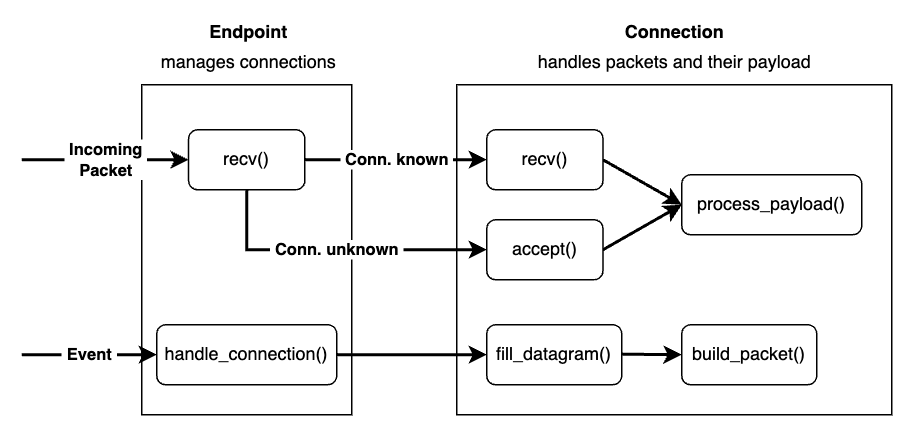
\includegraphics[width=1.0\linewidth]{img/lib_design.png}
    \end{subfigure}
    \caption{Rough Library Outline of Data Flow and Event Handling}
    \label{grafik_lib_design}
\end{figure}

\subsection{Initial packets} \label{initial_conn}

If the query yields no valid result however, the packet is considered to be of the initial type. Any other type results in an error and the
whole packet will be discarded. The endpoint now has to perform a number of steps to initialize the new connection and create all
necessary configurations. First, the initial keys are derived using rustls: \\
\inlinecode{let ikp = Keys::initial(Version::V1, \&head.dcid.id, Side::Server);} \\
With the resulting keyset, the header is decrypted (\ref{header_decrypt}) and the packet number, as well as the packet length fields are
populated with the decrypted values. Through using the \inlinecode{split()} fucntion of the \inlinecode{OctetsMut} object we are now
able to isolate the \inlinecode{payload\_cipher} and pass it to rustls
with the correct key to gain access to the decrypted frames contained within the packet.

\begin{codeblock}{lib.rs}{Rust}
    \begin{rustcode}
        let dec_len = {
            let decrypted_payload_raw = match ikp.remote.packet.decrypt_in_place(
                head.packet_num.into(),
                header_raw.as_ref(),
                payload_cipher.as_mut(),
            ) {
                Ok(p) => p,
                Err(error) => panic!("Error decrypting packet body {}", error),
            };
            decrypted_payload_raw.len()
        };
    \end{rustcode}
\end{codeblock}

When decrypting the payload, the decrypted data is always smaller than the cipher text. That is why \inlinecode{decrypt\_in\_place()}
returns only a part of the \inlinecode{payload\_cipher} as a slice.

After that, we have to initialize the QUIC transport parameters of our endpoint. Most of these parameters are set with default values
except for the original destination connection id(1), the initial source connection id(2) and the stateless reset token(3). (1) can
be obtained trivially from the decoded header, (2) has to be generated (\ref{handshake_cids}) randomly using \ref{connection_id_generation}
and (3) is generated using the hmac reset key and the previsouly generated initial source connection id.

\begin{codeblock}{lib.rs}{Rust}
    \begin{rustcode}
        let mut transport_config = transport_parameters::TransportConfig::default();
        transport_config
            .original_destination_connection_id(orig_dcid.id()) // (1)
            .initial_source_connection_id(initial_local_scid.id()) // (2)
            .stateless_reset_token( 
                token::StatelessResetToken::new(&self.hmac_reset_key, &initial_local_scid)
                    .token
                    .to_vec(), // (3)
            );
    \end{rustcode}
\end{codeblock}

With the transport configuration parameters being set, the tls session of type \\ 
\inlinecode{RustlsConnection::Server} can be initialized. In order to so it needs an \inlinecode{Arc} (a thread-safe reference-counting pointer)
to the server config, the QUIC version being used and the encoded transport parameters.

\begin{codeblock}{lib.rs}{Rust}
    \begin{rustcode}
        let conn = RustlsConnection::Server(
            rustls::quic::ServerConnection::new(
                std::sync::Arc::new(self.server_config.as_ref().unwrap().clone()),
                rustls::quic::Version::V1,
                transport_config_data.to_vec(),
            )
            .unwrap(),
        );
    \end{rustcode}
\end{codeblock}
        
After the tls session is initialized, a \inlinecode{Connection} object is created and inserted into the endpoints
connection vector. Additionally the new connection handle is created and can now be used to retrieve that connection. 
The packet and its header are then being passed into that new connection to the \inlinecode{accept()} function.

\begin{codeblock}{lib.rs}{Rust}
    \begin{rustcode}
        pub fn accept(
            &mut self,
            header: &Header,
            payload: &mut OctetsMut<'_>,
        ) -> Result<(), quic_error::Error> {
            self.process_payload(header, payload);

            self.generate_crypto_data();

            Ok(())
        }
    \end{rustcode}
\end{codeblock}

This function starts by processing the packet's payload (\ref{process_payload}), which contains a CRYPTO frame which in turn
contains the Client Hello message and generates the returning crypto data, in this case the Server Hello message using
the tls session and the function \inlinecode{write\_hs()}.

After returning from the connection, the endpoint returns a \inlinecode{Event} of type \inlinecode{NewConnection} which
contains the new connection handle.

\subsection{Known Connection} \label{known_conn}

If the incoming packet can be matched to an existing connection it is immediately passed into the corresponding object to
the \inlinecode{recv()} function. By using the \inlinecode{current\_space} identifier, the correct \inlinecode{PacketNumberSpace}
is retrieved. Within that object is the current keyset with which the header and payload are decrypted. The decrypted payload
is then passed on to \inlinecode{process\_payload()}.

\subsection{Processing Payload} \label{process_payload}

% process_payload(), read/write crypto data
To process a QUIC packets payload, every frame has to be decoded and processed in order. Firstly, the function checks for
every frame if it is ack eliciting. \\
\inlinecode{ack\_eliciting = !matches!(frame\_code, 0x00 | 0x02 | 0x03 | 0x1c | 0x1d);} \\
If the frame code is anything else than \inlinecode{PADDING}, \inlinecode{ACK}, and \inlinecode{CONNECTION\_CLOSE},
the packet requires an acknowledgement to be sent which is checked after the whole payload has been processed. The function
then loops over the buffer with each iteration extracting a single frame until all frames have been parsed.

\begin{codeblock}{lib.rs}{Rust}
    \begin{rustcode}
        match frame_code {
            0x00 => continue, //PADDING
            0x02 | 0x03 => {
                let _ack = AckFrame::from_bytes(&frame_code, payload);
            } //ACK
            0x05 => {
                let _stream_id = payload.get_varint().unwrap();
                let _application_protocol_error_code = payload.get_varint().unwrap();
            } //STOP_SENDING
            0x06 => {
                let crypto_frame = CryptoFrame::from_bytes(&frame_code, payload);
                self.process_crypto_data(&crypto_frame);
            } //CRYPTO
            [...] //all other frames
            _ => eprintln!(
                "Error while processing frames: unrecognised frame {:#x} at {:#x}",
                frame_code,
                payload.off()
            ),
        }
    \end{rustcode}
    \label{process_payload_code}
\end{codeblock}

Depending on the frame, a dedicated struct may be created except for frames which contain so few fields, that a dedicated struct
is not necessary, for example the \inlinecode{STOP\_SENDING} frame which only contains two fields. The resulting data may then be processed
accordingly. Crypto data is passed to \inlinecode{process\_crypto\_data()} which calls \inlinecode{read\_hs()} provided by the
\inlinecode{RustlsConnection} object. This function consumes the crypto data and prepares the according answer which is extracted
using \inlinecode{write\_hs()} after the payload has been processed in \inlinecode{accept()}.

\subsection{Event Handling}

The endpoint function \inlinecode{recv()} returns an \inlinecode{Event} which can then be acted upon in the applications interest. The
application may also choose to emit another event, such as \inlinecode{ConnectionClose}.

\begin{codeblock}{main.rs}{Rust}
    \begin{rustcode}
        let event = endpoint.recv();
        match event {
            Ok(event) => match event {
                Event::NewConnection(ch) => {
                    //maybe check if endpoint can handle more connections
                    let _ = endpoint.handle_connection(ch);
                }
                //[...] other events
                _ => (),
            },
            Err(error) => eprint!("{}", error),
        }
    \end{rustcode}
    \label{event_handling_main}
\end{codeblock}

It is then passed into the endpoint again, which takes the connection handle contained within, extracts the connection and calls
\inlinecode{fill\_datagram()}. Said method returns the length up to which the buffer has been written to. The \inlinecode{packet\_length}
is then used to slice the buffer and send the packet to the current remote address.

\begin{codeblock}{lib.rs (handle\_connection())}{Rust}
    \begin{rustcode}
        let connection = match self.connections.get_mut(connection_handle);

        let mut buffer = [0u8; 65535];

        let packet_length = connection.fill_datagram(&mut buffer).unwrap();

        let size = match self
            .socket
            .send_to(&buffer[..packet_length], connection.remote);
    \end{rustcode}
    \label{event_handling_endpoint}
\end{codeblock}

\subsection{Constructing Packets}

One UDP datagram may be filled with multiple, coalesced QUIC packets. If so, packets have to be ordered
by their packet number space with the lowest being the first. The function \inlinecode{fill\_datagram()} loops
through every packet number space and assembles a datagram with at least one packet.

\begin{codeblock}{lib.rs (fill\_datagram())}{Rust}
    \begin{rustcode}
        let mut size: usize = 0;

        for space_id in 0..(self.current_space + 1) {
            size += self.build_packet_in_space(&mut buffer[size..], space_id)?;
        }
    \end{rustcode}
    \label{fill_datagram}
\end{codeblock}

For every \inlinecode{PacketNumberSpace} the function \inlinecode{build\_packet\_in\_space()} is called which creates
and encodes the correct header, then populates the payload with a call to \\ \inlinecode{populate\_packet\_payload()} and
then encrypts the payload and the header. It also checks numerous edge cases, for example if the packet conforms to the
minimum size of 1200 bytes. The function \inlinecode{populate\_packet\_payload()} only checks for available data for
different frame types and encodes these. 

\begin{codeblock}{lib.rs (populate\_packet\_payload())}{Rust}
    \begin{rustcode}
        let mut size = 0;

        //CRYPTO
        if let Some(crypto_buffer) = &self.packet_spaces[packet_number_space].outgoing_crypto_data {
            if !crypto_buffer.is_empty() {
                size += match CryptoFrame::new(0, crypto_buffer.to_vec()).to_bytes(buf);
            }
        }

        //[...] other frame types, i.e. ACK, STREAM, ...
    \end{rustcode}
    \label{populate_packet_payload}
\end{codeblock}

\section{Error Handling}

Errors are handled on three different levels.
\begingroup
\renewcommand\labelenumi{(\theenumi)}
\begin{enumerate}
\item \textbf{QUIC Errors} as defined in Sec. 20 \cite{rfc9000}, including possible TLS errors, result in the appropriate
error code being sent via a CONNECTION\_CLOSE frame for example. All Error types except TLS errors are represented by an enum 
\ref{quic_errors}. TLS erros range from 0x0100 to 0x01ff and are handled outside of the enum.
\item \textbf{Application Errors} that result in connection termination may be thrown by any application via an event and
result in a \inlinecode{CONNECTION\_CLOSE} frame with type 0x1d which holds the application defined error code.
\item \textbf{Implementation Errors} are handled within the library, most often through the \inlinecode{Result<(), Error>} return
type and cover all possible scenarios. A self-defined \inlinecode{Error} contains a code and a reason. Error codes are consistent across
the whole library and defined in \inlinecode{quic\_error.rs}. For easier implementation a macro is used. \ref{quic_errors_self_defined}
\end{enumerate}
\endgroup

\begin{codeblock}{quic\_error.rs}{Rust}
    \begin{rustcode}
        enum QuicTransportErrors {
            NoError = 0x00,
            InternalError = 0x01,
            ConnectionRefused = 0x02,
            FlowControlError = 0x03,
            StreamLimitError = 0x04,
            StreamStateError = 0x05,
            // [...] 0x06 to 0x10
        }
    \end{rustcode}
    \label{quic_errors}
\end{codeblock}

\begin{codeblock}{quic\_error.rs}{Rust}
    \begin{rustcode}
        #[derive(Debug)]
        pub struct Error {
            code: u64,
            msg: String,
        }

        macro_rules! quic_error {
            ($name:ident, $code:expr) => {
                pub fn $name<T>(reason: T) -> Self
                where
                    T: Into<String>,
                {
                    Self {
                        code: $code,
                        msg: reason.into(),
                    }
                }
            };
        }

        impl Error {
            quic_error!(fatal, 0x00);
            quic_error!(unknown_connection, 0x01);
            quic_error!(socket_error, 0x02);
            [...] //Other Errors
        }
    \end{rustcode}
    \label{quic_errors_self_defined}
\end{codeblock}

%\section{Executing}

%tested code, testing with example application
%provide examples with quinn